\documentclass[12pt, a4paper]{report}
\usepackage[T1]{fontenc}
\usepackage[latin1]{inputenc}
\usepackage[english]{babel}
\usepackage{csquotes}
\usepackage{siunitx}
\usepackage{graphicx}
\usepackage{tipa} % for the \ark{} command
\usepackage{graphics} % for pdf, bitmapped graphics files
\usepackage{times} % assumes new font selection scheme installed
\usepackage{amsmath}
\usepackage{latexsym}
\usepackage{amscd}% for commutative diagrams
\usepackage{mathrsfs} %this package is for the script font \mathscr
\usepackage{relsize}
\usepackage{delarray}
\usepackage{pstricks}
\usepackage{theorem}
\usepackage{changepage}
\usepackage{euscript}
\usepackage{textcomp}
\usepackage{esvect}
\usepackage{parskip}
\usepackage{placeins}
\usepackage{subfigure}
\usepackage{array}
\usepackage{delarray}
\usepackage{stmaryrd}
\usepackage{fancyhdr}
\usepackage{graphpap}
\usepackage{makeidx}
\usepackage{enumerate}
\usepackage{esint}
\usepackage{datetime}
\usepackage{caption}
\usepackage{smartdiagram}
\usesmartdiagramlibrary{additions}
%Set Abstract Page
\usepackage{abstract}
\setlength{\absleftindent}{-5mm}
\setlength{\absrightindent}{-5mm}

%Colour definitions - put before TikZ
\usepackage{color}
\definecolor{igreen}{rgb}{0.0, 0.56, 0.0}
\usepackage{xcolor, colortbl}
\colorlet{gred}{-red!75!green!65!}
\colorlet{mamber}{-red!75!green!15!blue!50!}
\colorlet{grown}{-red!75!blue!20!green}
\colorlet{bled}{-red!85!blue!40!green!45!}
\colorlet{waters}{cyan!25} % Define color for the water
\colorlet{water}{cyan!25!green!20!} % Define color for the water
\definecolor{grin}{HTML}{00F9DE}
\usepackage{rotating}
\providecommand{\keywords}[1]{\textbf{\textit{Keywords---}} #1}

% For faint dotted table line
\usepackage{arydshln}
\setlength{\dashlinedash}{.4pt}
\setlength{\dashlinegap}{.8pt}

\usepackage{booktabs}
\usepackage{graphicx}
\graphicspath{ {images/} }
\usepackage{tikz}
\usepackage{tikz-3dplot}
\usepackage{pgfplots}
\pgfplotsset{compat=1.5}
\usetikzlibrary{
arrows,
arrows.meta,
automata,
backgrounds,
calc,
decorations,
decorations.pathmorphing,
decorations.pathreplacing,
decorations.fractals,
external,
fit,
matrix,
petri,
positioning,
shadows,
shapes,
shapes.multipart,
topaths,
intersections
}
\usepackage{eso-pic}
\def\ba{\begin{array}}
\def\ea{\end{array}}
\def\beann{\begin{eqnarray*}}
\def\eeann{\end{eqnarray*}}
\def\bea{\begin{eqnarray}}
\def\eea{\end{eqnarray}}
\def\bsy{\boldsymbol}
\def\gray#1{{\color{gray}#1}}

%% COUNTERS
\setcounter{MaxMatrixCols}{20}
\renewcommand{\thesection}{\arabic{section}}
\renewcommand{\thesection}{\thechapter.\number\numexpr\value{section}}
\renewcommand{\thesubsection}{\thesection.\number\numexpr\value{subsection}}
%%For changemargin
\def\quote{\list{}{\rightmargin\leftmargin}\item[]}
\let\endquote=\endlist 
\def\changemargin#1#2{\list{}{\rightmargin#2\leftmargin#1}\item[]}
\let\endchangemargin=\endlist 
\makeatletter
\newlength\qvec@height
\newlength\qvec@depth
\newlength\qvec@width
\newcommand{\qvec}[2][]{
    \settoheight{\qvec@height}{$#2$}
    \settodepth{\qvec@depth}{$#2$}
    \settowidth{\qvec@width}{$#2$}
  \def\qvec@arg{#1}
  \raisebox{.2ex}{\raisebox{\qvec@height}{\rlap{% 
    \kern.05em
    \begin{tikzpicture}[scale=1,shorten >=-3pt,shorten <=-3pt]
    \pgfsetroundcap
    \coordinate (Stx) at (.05em,0) ;
		\coordinate (Arx) at (\qvec@width-.05em,0) ;
    \draw[->](Stx) to[bend left] (Arx);
    \end{tikzpicture}
  }}}
  #2
}
\makeatother
\makeatletter
\newlength\pvec@height
\newlength\pvec@depth
\newlength\pvec@width
\newcommand{\pvec}[2][]{
    \settoheight{\pvec@height}{$#2$}
    \settodepth{\pvec@depth}{$#2$}
    \settowidth{\pvec@width}{$#2$}
  \def\pvec@arg{#1}
  \raisebox{.2ex}{\raisebox{\pvec@height}{\rlap{% 
    \kern.05em
    \begin{tikzpicture}[scale=1,shorten >=-3pt,shorten <=-3pt]
    \pgfsetroundcap
    \coordinate (Stx) at (.05em,0) ;
		\coordinate (Arx) at (\pvec@width-.05em,0) ;
    \draw[->](Stx) to[bend right] (Arx);
    \end{tikzpicture}
  }}}
  #2
}
\makeatother
\makeatletter
\newlength\vvec@height%
\newlength\vvec@depth%
\newlength\vvec@width%
\newcommand{\vvec}[2][]{%
  \ifmmode%
    \settoheight{\vvec@height}{$#2$}%
    \settodepth{\vvec@depth}{$#2$}%
    \settowidth{\vvec@width}{$#2$}%
  \else 
    \settoheight{\vvec@height}{#2}%
    \settodepth{\vvec@depth}{#2}%
    \settowidth{\vvec@width}{#2}%
  \fi%
  \def\vvec@arg{#1}%
  \def\vvec@dd{:}%
  \def\vvec@d{.}%
  \raisebox{.2ex}{\raisebox{\vvec@height}{\rlap{%
    \kern.05em%
    \begin{tikzpicture}[scale=1]
    \pgfsetroundcap
    \draw (.05em,0)--(\vvec@width-.05em,0);
    \draw (\vvec@width-.05em,0)--(\vvec@width-.15em, .075em);
    \draw (\vvec@width-.05em,0)--(\vvec@width-.15em,-.075em);
    \ifx\vvec@arg\vvec@d%
      \fill(\vvec@width*.45,.5ex) circle (.5pt);%
    \else\ifx\vvec@arg\vvec@dd%
      \fill(\vvec@width*.30,.5ex) circle (.5pt);%
      \fill(\vvec@width*.65,.5ex) circle (.5pt);%
    \fi\fi%
    \end{tikzpicture}%
  }}}%
  #2%
}
\makeatother
\def\ba{\begin{array}}
\def\ea{\end{array}}
\def\beann{\begin{eqnarray*}}
\def\eeann{\end{eqnarray*}}
\def\bea{\begin{eqnarray}}
\def\eea{\end{eqnarray}}
\def\bsy{\boldsymbol}
\def\gray#1{{\color{gray}#1}}
\usepackage{titlesec}
\usepackage{multirow}
%To reference within text
\usepackage{hyperref}
\usepackage{lipsum}
\usepackage{tikz-cd}
\usepackage{float}
\usepackage{titling}
\usepackage{epigraph}
\usepackage[title, titletoc]{appendix}
\setlength\epigraphwidth{8cm}
\setlength\epigraphrule{0pt}

\titleformat{\chapter}{\normalfont\LARGE}{\thechapter\,$\vert$}{20pt}{\LARGE}{\setcounter{chapter}{0}}
\setlength{\headheight}{15pt}
\titlespacing*{\chapter}{0pt}{-70pt}{40pt} %Move chapter titles up

% Title page logos:
\makeatletter
\newcommand\BackgroundPicturea[3]{
	\setlength{\unitlength}{1pt}
	\put(0,\strip@pt\paperheight){
		\parbox[t]{\paperwidth}{
			\vspace{#2}\hspace{#3}
			\mbox{\includegraphics[scale=0.5]{#1}}
}}}
\newcommand\BackgroundPictureb[3]{
	\setlength{\unitlength}{1pt}
	\put(0,\strip@pt\paperheight){
		\parbox[t]{\paperwidth}{
			\vspace{#2}\hspace{#3}
			\mbox{\includegraphics[scale=0.3]{#1}}
}}}
\makeatother

% For my abbreviations
\newcommand{\abbrlabel}[1]{\makebox[3cm][l]{\textbf{#1}\ \dotfill}}
\newenvironment{abbreviations}{\begin{list}{}{\renewcommand{\makelabel}{\abbrlabel}}}{\end{list}}

% Line Spacing
\usepackage{setspace}

%Set of command is for the changemargin environment
\def\quote{\list{}{\rightmargin\leftmargin}\item[]}
\let\endquote=\endlist 
\def\changemargin#1#2{\list{}{\rightmargin#2\leftmargin#1}\item[]}
\let\endchangemargin=\endlist

%Replace Contents to Table of Contents	
\addto\captionsenglish{
	\renewcommand{\contentsname}%
	{Table of Contents}
	\setcounter{tocdepth}{3}% Include \subsubsection in ToC
	\setcounter{secnumdepth}{3}% Number \subsubsection in ToC
	}
\renewcommand{\listfigurename}{List of Figures}
\renewcommand{\listtablename}{List of Tables}

\bibliographystyle{unsrtnat}
\usepackage[
    natbib=true,
    style=numeric,
    sorting=none
]{biblatex}
\addbibresource{references.bib}


\hypersetup{pdftitle = Thesis, pdfauthor = {First Last}, pdfstartview=FitH, pdfkeywords = essay, pdfpagemode=FullScreen, colorlinks, anchorcolor = red, citecolor = blue, urlcolor=blue, filecolor=green, linkcolor=red, plainpages=false}

\pagestyle{fancy}
\rhead{\thepage}
\chead{}
\lhead{\nouppercase{\rightmark}}
\lfoot{\date{}}
\cfoot{}
\rfoot{}

% Top and Bottom Line Rules
\renewcommand{\headrulewidth}{0.4pt}
\renewcommand{\footrulewidth}{0.4pt}
\fancyheadoffset{9pt}
\fancyfootoffset{9pt}

% Line spacing
\renewcommand{\baselinestretch}{1.0}

%################################################################################################
% title
\title{
{Achromatic Composite Waveplates in the Terahertz Frequency Range}\\
{\large Institution of THz}\\
%{
\includegraphics[]{tcVF8.jpg}}
}
\author{ALEX}
\date{10 10 1910}
% title
%################################################################################################

% beginning of the end ...
\begin{document}
\maketitle

%################################################################################################
% frontmatter
\chapter*{Abstract}

\chapter*{Dedication?}

\chapter*{Declaration?}

\chapter*{Acknowledgements}
I want to thank Jan :)

\tableofcontents

\listoffigures

% frontmatter
%################################################################################################

\chapter{Introduction}
\section{Brief introduction to THz}
On the electromagnetic spectrum, terahertz (THz) refers to electromagnetic waves with photon energies ranging from around 1 to \SI{100}{\milli \electronvolt}. This corresponds to frequencies roughly around \SI{240}{\giga \hertz} for the lower energy photons and \SI{24}{\tera \hertz} for photons with an energy of \SI{100}{\milli \electronvolt}.


\section{Motivation for this work}
Polarization control is an important aspect of optics. etc https://en.wikipedia.org/wiki/BB84
- usages of waveplates
- Folder with examples from litterature


\chapter{THz Time Domain Spectroscopy}
\section{combine 2 and 4, not sure what to put here yet}

\begin{tikzpicture}
	\begin{axis}[
	axis line style = very thick,
	%every tick/.style={black, very thick},
	xlabel=Time (yrs),
    ylabel=Work done (\SI{}{Nm}),
    anchor=origin,
    legend entries={Alex}
	]
	
	\addplot +[thin, mark options={scale=0}] table [
	x expr=\thisrowno{0}/1000, 
	y expr=\thisrowno{2}*1000, col sep=comma]
	{plot_data/2020-10-15T15-22-54.690036-vertical-122.000 mm.csv};
	
	\end{axis}
\end{tikzpicture}


\chapter{Theory}
In this chapter we will introduce the basic principles required to understand what waveplates are and how they work in general. Simply put the purpose of a waveplate is to change the polarization of EM waves, most commonly by using a birefringent material. The polarization of EM waves, birefringence and how the waveplates work are explained in more detail in the sections \ref{sec:polellipse}, \ref{sec:birefringence} and \ref{sec:waveplates}. This change of the polarization state caused by the waveplate, and the state itself, can be described mathematically using Jones calculus or almost equivalently using Mueller calculus, which will be shown in section \ref{sec:mathdescription}. Finally, this leads to the description of the design and the design optimization problem in the last section (\ref{sec:design}) of this chapter.


\section{The polarization ellipse}
\label{sec:polellipse}
There are several ways to describe the polarization state of EM-waves. One of them is the polarization ellipse which is a geometrical representation of the polarization. This remained the only satisfactory way to visualize the different polarization states for almost the entire 19\textsuperscript{th} century, although it is not very practical for carrying out calculations. At the end of the century another representation was proposed by Henri Poincaré, now known as the Poincaré sphere, which could be used for both calculations and visualization of the polarization states \cite{Collett2008VisualizationSphere}. Poincaré's representation will be explained in section \ref{sec:muellercalc}. The polarization ellipse can be derived either directly from a solution to the EM-wave equation or starting from Maxwell's equations.  It is practical to start from Maxwell's equations, since they are used for derivations later on in this work and almost all equations used originate from them. In differential form Maxwell's equations are given by: 
\par
\noindent\begin{minipage}{.5\linewidth}
\begin{align}
    \bm{\nabla}\cdot\bm{D} &=\rho_{f}\;,\label{eq:maxwell1}
    \vphantom{\frac{\partial\bm{B}}{\partial t}}\\
    \bm{\nabla}\cdot\bm{B} &=0\;,\vphantom{\frac{\partial\bm{B}}{\partial t}}\label{eq:maxwell2}
\end{align}
\end{minipage}%
\begin{minipage}{.5\linewidth}
\begin{align}
    \bm{\nabla}\times\bm{E} &=-\frac{\partial\bm{B}}{\partial t}\;,\label{eq:maxwell3}
    \\
    \bm{\nabla}\times\bm{H} &=\bm{J}_f
    +\frac{\partial\bm{D}}{\partial t}\;,\label{eq:maxwell4}
\end{align}
\end{minipage}
\newline

where $\bm{E}, \bm{H}$ denote the electric and magnetizing fields respectively,  $\bm{D}=\hat{\epsilon} \bm{E}$ is the electric displacement, $\hat{\epsilon}$ is the permittivity of the material and t denotes time. The materials used in this work are non magnetic, which means that the magnetic and magnetizing fields are proportional: $\bm{B} = \mu_0 \bm{H}$, where $\mu_0$ denotes the vacuum permeability. $\rho_f, \bm{J}_f$ is the free charge and current density respectively. Usually in optics there are no free charge carriers or free currents, which is also the case for all materials in this work, so we set $\rho_f=\bm{J}_f=0$ \cite{Roth2019Optik}. If we then also assume that the materials are homogeneous so that $\hat{\epsilon}$ does not depend on position, then we can reduce equations \ref{eq:maxwell1}-\ref{eq:maxwell4} to the following:

\noindent\begin{minipage}{.5\linewidth}
\begin{align}
    \bm{\nabla}\cdot \bm{E} &=0\;,\label{eq:maxwell1reduced}
    \vphantom{\frac{\partial\bm{B}}{\partial t}}\\
    \bm{\nabla}\cdot\bm{B} &=0\;,\vphantom{\frac{\partial\bm{B}}{\partial t}}\label{eq:maxwell2reduced}
\end{align}
\end{minipage}%
\begin{minipage}{.5\linewidth}
\begin{align}
    \bm{\nabla}\times\bm{E} &=-\frac{\partial\bm{B}}{\partial t}\;,\label{eq:maxwell3reduced}
    \\
    \bm{\nabla}\times\bm{B} &=\mu_0 \hat{\epsilon} \frac{\partial\bm{E}}{\partial t}\;,\label{eq:maxwell4reduced}
\end{align}
\end{minipage}
\newline

Applying $\bm{\nabla}\times$ to equation \ref{eq:maxwell3reduced} and with equation \ref{eq:maxwell4reduced} we decouple $\bm{E}$ and $\bm{B}$: 
\begin{equation}
    \bm{\nabla}\times \bm{\nabla}\times \bm{E} = -\mu_0 \hat{\epsilon} \frac{\partial^2\bm{E}}{\partial t^2}
\end{equation}
Then using the vector calculus identity: $\bm{\nabla}\times \bm{\nabla}\times \bm{F} = \bm{\nabla} \left( \bm{\nabla} \cdot \bm{F} \right) - \bm{\nabla}^2 \bm{F}$, for any function $\bm{F}$, together with equation \ref{eq:maxwell1reduced} we get the EM-wave equation: \footnote{We neglect the magnetic field, since we are only concerned with non magnetic materials in this work. But the derivation of the wave equation for the magnetic field would be exactly the same}
\begin{equation}
    \label{eq:waveeq}
    \bm{\nabla}^2 \bm{E} = \mu_0 \hat{\epsilon} \frac{\partial^2\bm{E}}{\partial t^2}
\end{equation}
or in frequency space $(\partial_t \xrightarrow{\mathscr{F}} i\omega)$:
\begin{equation}
    \label{eq:waveeqfreq}
    \bm{\nabla}^2 \bm{E} = -\mu_0 \hat{\epsilon} \omega^2 \bm{E},
\end{equation}
where $\omega$ is the angular frequency.
A solution to the wave equation is a coherent plane wave at frequency $\omega$ which is given by: 
\begin{equation}
    \label{eq:planewave}
    \bm{E} = \bm{E_0} e^{i(\bm{k}\bm{r} - \omega t)},
\end{equation}
where $\bm{r}$ and $\bm{k}$ denote the position and wave vector respectively and $\bm{E_0}$ denotes the maximum amplitude of the wave. If we assume the wave propagates along the z-direction in a Cartesian coordinate system, then the amplitude will be orthogonal to the z-direction, i.e a transverse wave. This follows directly from equation \ref{eq:maxwell1reduced}. From the wave equation in frequency space we then find the requirement that the wave number, which is the magnitude of the wave vector, and the angular frequency are related by:
\begin{equation}
    k = \sqrt{\mu_0 \hat{\epsilon}} \omega
\end{equation}
The phase velocity of the wave can then be expressed as:
\begin{equation}
    v = \frac{\omega}{k} = \frac{1}{\sqrt{\mu_0 \hat{\epsilon}}} = \frac{c}{n},\:n = \sqrt{\frac{\hat{\epsilon}}{\epsilon_0}},
\end{equation}
where $c$, $\epsilon_0$ and $n$ is the speed of light in vacuum, vacuum permittivity and refractive index respectively.
So that from the wave equation we get two decoupled wave equations, each describing an oscillation in the x-z plane and the y-z plane. This is also known as Fresnel's wave theory which was proposed and verified experimentally around 1820 by Augustin-Jean Fresnel and François Arago, more than 40 years before Maxwell's equations were published \cite{Collett2009FieldPolarization,Jackson1998ClassicalEdition}.
This means equation \ref{eq:planewave} consists of only two perpendicular components. Additionally, if we consider that Maxwell's equations \ref{eq:maxwell1reduced}-\ref{eq:maxwell4reduced} are all linear and real, then it follows that the real part of any particular solution is also a solution to the wave equation. \footnote{This only works if the equations are real. For example, Schrödinger's equation is linear but complex, therefore even if $\psi$ is a solution $\operatorname{Re}(\psi)$ and $\operatorname{Im}(\psi)$ are not.} We can then write equation \ref{eq:planewave} as two sinusoidal waves:
\begin{equation}
\label{eq:plane_wave_realparts}
\begin{aligned}
    E_x(z, t) = E_{0x}\cos(kz-\omega t + \delta_x) \\
    E_y(z, t) = E_{0y}\cos(kz-\omega t + \delta_y), 
\end{aligned}
\end{equation}
where $\delta_x$ and $\delta_y$ are arbitrary phases. Depending on the values of $E_{0x}, E_{0y}$ and the relative phase or simply phase, which is $\delta = \delta_y - \delta_x$, we get different polarization states. Figure \ref{fig:Ex_Ey_planewaves} shows the real parts of the two plane wave components for a wave traveling along the z-direction when $\delta=0$ and $E_{0x}=E_{0y}$.

\begin{figure}[h]
    \centering
    \includestandalone{3_chapter03/tikz_e_wave}
    \caption{This figure shows the two sinusoidal waves given in equation \ref{eq:plane_wave_realparts}, which are the real parts of the plane wave components. Both waves have the same amplitude and phase.}
    \label{fig:Ex_Ey_planewaves}
\end{figure}

From here we can visualize the different polarization states, that is the different directions the electrical field, or simply the light, can oscillate in. If the light is confined to a plane along the direction of propagation it is said to be linearly polarized (LP). An example of this is shown in figure \ref{fig:E_planewave}, where the polarization plane is at an angle of \SI{45}{\degree} relative to the x-axis. 

\begin{figure}[h]
    \centering
    \includestandalone[scale=1.1]{3_chapter03/tikz_linear_pol}
    \caption{The black curve shows the superposition of the two sinusoidal waves from equation \ref{eq:plane_wave_realparts}, which is the same as the real part of a LP plane wave at an angle of \SI{45}{\degree} to the x-axis. In addition, the horizontal and the vertical components of the field vector are shown as the red and blue curves respectively.}
    \label{fig:E_planewave}
\end{figure}

Now, if $\delta$ is exactly $\nicefrac{\pi}{2}$ and $E_{0x} = E_{0y}$, then we get the case shown to the right in figure \ref{fig:circ_pol_planewave}. A field with this kind of polarization traces out a circle as time passes for a fixed position in space. On the other hand, if we keep time fixed then the field vector describes a helix along the direction of propagation. This means the field only changes direction but not its magnitude. This type of polarization is therefore called circular polarization (CP). Additionally, because we can trace out a circle in two different directions (clockwise or counterclockwise) we therefore get two different types of circular polarizations. These two types are called right CP (RCP) or left CP (LCP) depending on the direction the circle is traced out, so either in a left- or right-handed sense. This is called the handedness of the light, which can be determined using the right hand rule. For that we fix the right hand at a point on the helix and point the thumb away from the receiver, that is against the direction of propagation. Then the light is right-handed if the helix is traced out in the direction of the other fingers as time revolves, otherwise it is left-handed. The light shown to the left of figure \ref{fig:circ_pol_planewave} is therefore left-handed while the example on the right side of figure \ref{fig:circ_pol_planewave} shows right-handed CP light. The reason why we have two types of CP in the first place, is because of the fact that one component can lead the other, as we can see in figure \ref{fig:circ_pol_planewave}. Where for RCP the horizontal component leads the vertical one by a quarter period ($\delta = -\nicefrac{\pi}{2}$), for LCP it is the other way around and $\delta = \nicefrac{\pi}{2}$. 

\begin{figure}[h]
\centering
    \begin{subfigure}
        \centering
        \includestandalone[scale=0.8]{3_chapter03/tikz_circ_pol_lh}
    \end{subfigure}
    \begin{subfigure}
        \centering
        \includestandalone[scale=0.8]{3_chapter03/tikz_circ_pol_rh}
    \end{subfigure}
    \caption{The left figure shows an example of LCP light and the right figure RCP light. Furthermore, handedness originates from one component leading the other. In the case of LCP light the vertical component leads the horizontal component and vice versa for RCP light.}
    \label{fig:circ_pol_planewave}
\end{figure}

\newpage

Finally, the last polarization state we have not mentioned yet, even though it is in fact the most general, is the elliptical polarization state. The polarization states we have dealt with so far have all been limiting cases of this state. For a fixed position this is fairly simple to visualize geometrically; LP light traces out a line while CP light traces out a circle, both of these shapes are degenerate forms of an ellipse. A summary of the different degenerate states and the corresponding amplitude and phase combinations are shown in table \ref{tab:pol_state_summary}, which is divided into three parts with a pair of states in each. At the top there str the linear horizontal/vertical polarization (LHP/LVP) stated, the linear $\pm\SI{45}{\degree}$ polarization ($L_{\pm45}P$) states are in the middle and the CP states are at the bottom. The last column shows the corresponding degenerate ellipse figure for each state.

\begin{table}
    \centering
    \includestandalone{3_chapter03/pol_summary_table}
    \caption{Summary of the different degenerate polarization states, with corresponding conditions figures. The first four states are linearly polarized at different angles relative to the x-axis; $\SI{0}{\degree}$, $\SI{90}{\degree}$, $\SI{45}{\degree}$ and $\SI{-45}{\degree}$ respectively. The last two are the RCP and LCP states.}
    \label{tab:pol_state_summary}
\end{table}

We can also realize this mathematically by eliminating the time and position dependency of the two components in equation \ref{fig:Ex_Ey_planewaves}, so that we get:

\begin{equation}
    \centering
    \frac{1}{\sin^2 \delta} \left[ \left(\frac{E_x}{E_{0x}}\right)^2+\left(\frac{E_y}{E_{0y}}\right)^2-2\frac{E_x E_y}{E_{0x} E_{0y}}\cos \delta \right]=1,
\end{equation}

which describes an ellipse in its nonstandard form. 

\begin{figure}[h]
    \centering
    \includestandalone{3_chapter03/tikz_pol_ellipse}
    \caption{}
    \label{fig:pol_ellipse}
\end{figure}

To finish off the section we will talk about the conventions. Tomorrow, again ...

\section{Birefringence}
\label{sec:birefringence}
Birefringence is the material property responsible for the phenomenon of double refraction. This phenomenon was observed for the first time in calcite crystals by the Danish scientist Rasmus Bartholin in 1669 \cite{RasmusBartholin1669ExperimentaDetegitur, Restaino2015PolarizationDevices}. The effect of double refraction on a light beam passing through a birefringent material is relatively easy to show. One can simply place a birefringent crystal on top of some text, as it is shown in figure \ref{fig:3birefringence}. Two images of the text become visible through the crystal and each image is shifted by a different amount. These images are not simply reflections at the crystal-air interface, since the images are brighter compared to images formed through reflections, and they are even visible when looking down directly from above. Also if the crystal is rotated then one of the pictures will be stationary, while the other one will circle around the stationary image. The same effect can be illustrated by sending an unpolarized laser beam through the crystal. The beam is split in two as it propagates through the crystal. Another effect of birefringence, which is more subtle, is that each of the two beams exiting the crystal will be polarized perpendicular to each other \cite{Roth2019Optik}.

\begin{figure}[h]
    \centering
    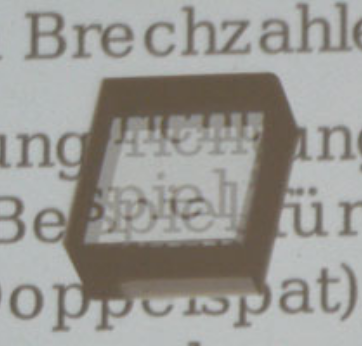
\includegraphics[scale=0.35]{images/3_chapter03/birefringence.png}
    \caption{A calcite crystal placed on top of some text. This demonstrates the effect of birefringence on the original image seen through the crystal. \cite{Roth2019Optik}}
    \label{fig:3birefringence}
\end{figure}

\subsection{Natural}

\subsection{Form birefringence}

\section{Waveplates}
\label{sec:waveplates}

\section{Mathematical description}
\label{sec:mathdescription}

\subsection{Boundary conditions}

\subsection{Jones calculus}

\subsection{Mueller calculus}
\label{sec:muellercalc}

\section{Design description}
\label{sec:design}

\subsection{Optimization?}
- describe algorithm


\chapter{Experimental setup and procedure}
\section{Experimental Setup}
We want to measure in two ranges because of birefringence and stuff so we need two setups hehe:

\subsection{THz setup}
Hello :)
\begin{figure}[h]
    \centering
    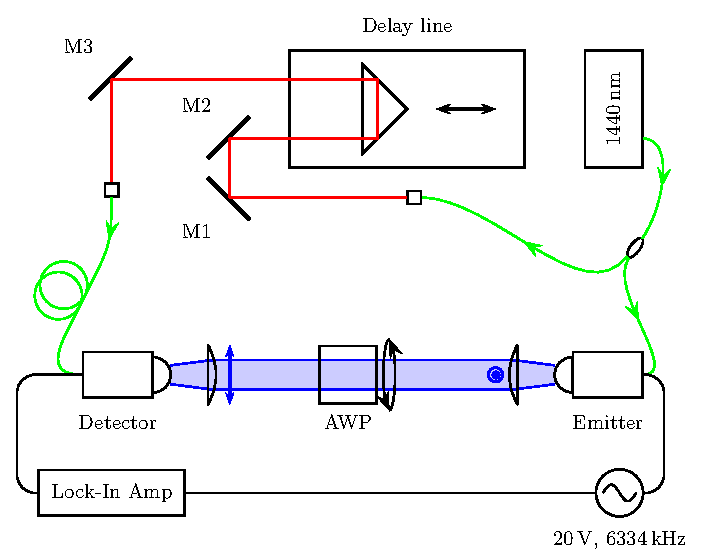
\includegraphics{images/4_chapter04/Setup1_TDS.pdf}
    \caption{THz setup : ))}
    \label{fig:THz_setup}
\end{figure}


\subsection{GHz setup???}
\begin{figure}[h]
    \centering
    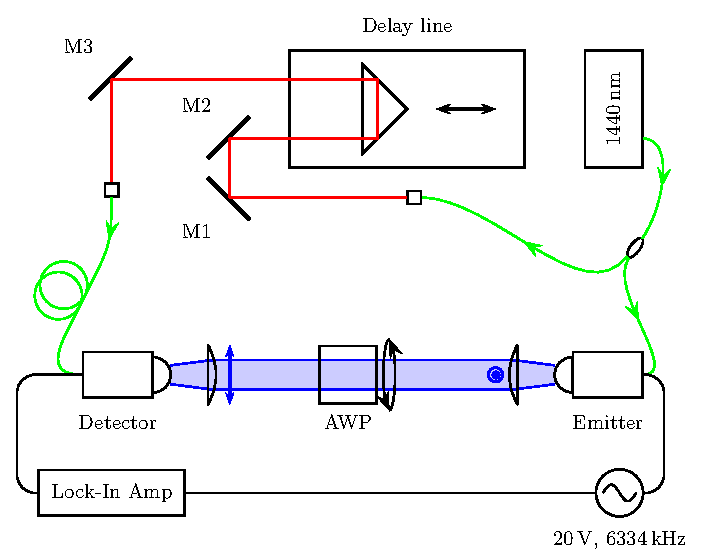
\includegraphics{images/4_chapter04/Setup1_TDS.pdf}
    \caption{Placeholder for GHz setup if I get one ...}
    \label{fig:GHz_setup}
\end{figure}
Halp



\chapter{Results}
\section{Waveplate sample types}
\subsection{3D printed}
\subsection{SLE}
\subsection{Ceramic 3D printing}
\section{Results and discussion}
\subsection{Simulation}
\subsubsection{Fabrication error}
\subsection{CST}


\chapter{Conclusion}
- Summary: We proposed a new loss function based on the Jones calculus which was then used in the design process. 
\newline
    - Add about formbirefringence
    \newline
    - Also compared the optimization result to another result obtained with a different objective function. (Ceramic)
\newline
We tested the design obtained from optimizing the loss function by 3D printing and subsequently characterizing the waveplate/structure. It was not done by us, not sure if needs to be mentioned again. 
\newline
- Large deviation but we could identify a likely cause. We did see a broadband response compared to a single waveplate.
\newline
- Outlook: What more can be done? What I'm doing now lol. We can get better results fairly easy...


\appendix
\chapter{Clunky stuff}
\section{Polarization ellipse derivation}
\label{sec:deriv_pol_ellipse}
Setting $kz-\omega t=\tau$ in the plane wave equations:
\begin{equation}
\begin{aligned}
    E_x(z, t) = E_{0x}\cos(\tau + \delta_x) \\
    E_y(z, t) = E_{0y}\cos(\tau + \delta_y).
\end{aligned}
\end{equation}
In order to eliminate $\tau$ we write the previous equations as:
\begin{equation}
\begin{aligned}
    \frac{E_x}{E_{0x}} = \cos(\tau)\cos(\delta_x) - \sin(\tau)\sin(\delta_x)\\
    \frac{E_y}{E_{0y}} = \cos(\tau)\cos(\delta_y) - \sin(\tau)\sin(\delta_y).
\end{aligned}
\end{equation}
Multiplying by $\cos(\delta_{x,y})$, $\sin(\delta_{x,y})$ subtracting and using trig. angle difference formulas we get:
\begin{equation}
\begin{aligned}
    \frac{E_x}{E_{0x}}\sin(\delta_y) - \frac{E_y}{E_{0y}}\sin(\delta_x) = \cos(\tau)\sin(\delta_y-\delta_x)\\
    \frac{E_x}{E_{0x}}\cos(\delta_y) - \frac{E_y}{E_{0y}}\cos(\delta_x) = \sin(\tau)\sin(\delta_y-\delta_x).
\end{aligned}
\end{equation}
Squaring and adding these two equations gives:
\begin{equation}
    \left(\frac{E_x}{E_{0x}}\right)^2+\left(\frac{E_y}{E_{0y}}\right)^2-2\frac{E_x E_y}{E_{0x} E_{0y}}\cos \delta =\sin^2 \delta,
\end{equation}
with $\delta=\delta_y-\delta_x$, which is the polarization ellipse equation.

%\section{Index ellipsoid procedure}
%\label{sec:index_ellipse_proof}
% TODO remove? yes. (done)
% laser book

\section{Effective permittivity inequality}
\label{sec:bf_proof}
We want to show that $\epsilon_{s}<\epsilon_{p}$, where $\epsilon_{s}$ and $\epsilon_{p}$ are given in equation \ref{eq:rytov_2nd_order_final}. We assume that $1\leq\epsilon\leq4$ and that the ratio $r=\frac{d}{\lambda}$ is less than $0.6$ which is reasonable considering the condition stated in equation \ref{eq:rytov_cond1}. In order to slightly simplify the equations we can measure lengths in units of $d$ this means that $a+b=1$ or setting $a=f$ we end up with the following inequality we want to show:
\begin{equation}
    \label{eq:inequality_proof}
    0<1+\frac{\tilde{\epsilon}_{p}-\tilde{\epsilon}_{s}}{f^2(1-f)^2(\epsilon-1)^2c}-\frac{\tilde{\epsilon}_{p}\tilde{\epsilon}_{s}^3}{\epsilon^2},\quad c=\frac{1}{3}r^2\pi^2.
\end{equation}

Although, showing that this is true is fairly lengthy, we therefore only briefly describe the underlying idea. Since $\epsilon$ is bounded by $1$ and $4$ we can show that the right side of equation \ref{eq:inequality_proof}, which is a function of $\epsilon$ and $f$, is decreasing or increasing on some subset of the interval or the full interval if possible. If the right side is found to be increasing(decreasing) then we can simply show that the inequality is true at the lower(upper) bound of the interval. To show that the function is increasing(decreasing) we calculate the derivative with right to $\epsilon$ and show that it is strictly positive(negative), this gives us a new reduced inequality. Since equation \ref{eq:inequality_proof} is a polynomial the process will eventually terminate and we obtain simple inequalities for different subsections of the interval $[1,4]$. Doing this we were able to show that the inequality given in \ref{eq:inequality_proof} is true on the given interval and for all $f$ in $[0,1]$.

% Jan measurement setup (done)
\section{Transmission minimum of diattenuating linear retarder} 
\label{sec:transmission_min}
The setup consists of a linear horizontal polarizer $\hat{T}_{DL}(\psi=0, p_1=1, 0)$, linear diattenuating retarder (waveplate) $\hat{T}_{RDL}(\psi, \Delta, p_1, p_2)$ and another linear horizontal polarizer $\hat{T}_{DL}(\psi=0, p_1=1, 0)$ in the given order. The input is a normalized horizontal linear state $\bm{\mathcal{E}}_{\SI{0}{\degree}}$. The intensity of the output is then simply $I_o=T_{1,1}(T_{1,1})^*$, requiring $I_o\overset{!}{=}0$ we get the following:
\begin{equation}
    0=(p_1c_\psi^2e^{i\Delta/2}+p_2s_\psi^2e^{-i\Delta/2})(p_1c_\psi^2e^{-i\Delta/2}+p_2s_\psi^2e^{i\Delta/2}).
\end{equation}
Simplifying:
\begin{equation}
    \label{eq:trans_min_app}
    -2p_1p_2c_\Delta = p_1^2\left(\frac{c_\psi}{s_\psi}\right)^2 + p_2^2\left(\frac{s_\psi}{c_\psi}\right)^2
\end{equation}
The image of LHS is the interval $\left[-2p_1p_2, 2p_1p_2\right]$ while the image of the RHS is $\left[2p_1p_2, \infty\right)$. This means that equation \ref{eq:trans_min_app} only has a solution when
\begin{equation}
    c_\Delta=-1
\end{equation}
and
\begin{equation}
    2p_1p_2 = p_1^2\left(\frac{c_\psi}{s_\psi}\right)^2 + p_2^2\left(\frac{s_\psi}{c_\psi}\right)^2.
\end{equation}
From the first equation it follows that $\Delta=\pi$, $(\Delta \in [0,\pi])$ and the second equation is solved by:
\begin{equation}
    \label{eq:psi_min}
    \psi = \arctan \sqrt{\frac{p_2}{p_1}},
\end{equation}
that is, the intensity is zero for this $\psi=\psi_{min}$ given by equation \ref{eq:psi_min}.

\section{Basin-hopping algorithm}
\label{sec:basin_hopping_algo}

Basin-hopping is a stochastic algorithm which is used in global optimization problems and was first developed to solve problems in chemical physics \cite{Wales1997}. It is well suited for the optimization problems presented in this work, since it is an effective algorithm in the case of high dimensional smooth nonlinear loss functions $L(x)$ with multiple optima separated by large barriers \cite{Olson2012, Wu2020}. The algorithm mainly consists of cycling through three steps until some stop criterion is fulfilled. First a perturbation of a candidate solution is performed, then a local search is applied to the perturbed solution and then finally the coordinates are accepted or rejected based on the minimized function value. The associated pseudocode is shown in algorithm \ref{algo_bh}. 

\begin{algorithm}[H]
    \SetAlgoLined
    \SetKwFunction{LOCALSEARCH}{LOCALSEARCH}\SetKwFunction{STOP}{STOP}\SetKwFunction{PERTURB}{PERTURB}
    \SetKwFunction{METROPOLIS}{METROPOLIS}
    \SetKw{KwOr}{or}
    \SetKwData{NS}{not satisfied} \SetKwData{RP}{random initial point in variable space}
    
    $i \leftarrow 0$\;
    $x_i \leftarrow $ \RP\;
    $y_i \leftarrow $ \LOCALSEARCH{$x_i$}\;
    \While{\STOP \NS}{
        $x_{i+1} \leftarrow $ \PERTURB{$y_i$}\;
        $y_{i+1} \leftarrow $ \LOCALSEARCH{$x_i$}\;
        \If{$L(y_{i+1})<L(y_i)$ \KwOr{} \METROPOLIS{$y_{i+1}, y_i$}}{
            $i \leftarrow i+1$\;
        }
    }


\caption{Basin-hopping pseudocode}\label{algo_bh}
\end{algorithm}

Since we can not determine if the global minimum has actually been found for stochastic global optimization problems the \texttt{STOP} criterion is simply a number of iterations. The result is then the lowest minimum found. The additional acceptance criterion \texttt{METROPOLIS} is true with a probability $P(y_{i+1}, y_i)$ given by the following:
\begin{equation}
    P(y_{i+1}, y_i) = \exp\left(\frac{L(y_{i})-L(y_{i+1})}{T} \right),
\end{equation}
where $T$ is known as the temperature and is a user defined parameter which should be set similar to the average function value difference between local minima \cite{ScipyBH}. The \texttt{LOCALSEARCH} step is in our case perfomed by the L-BFGS-B local optimization routine which is a quasi-Newton algorithm and allows the specification of bounds \cite{Byrd1995}. \texttt{PERTURB} is responsible for taking a step in variable space with a stepsize $\tau$ which is another user defined parameter. $\tau$ is an important parameter in Basin-hopping and depends on the optimization problem. The step is chosen uniformly in the region from $x-\tau$ to $x+\tau$, in each dimension. The Python implementation of the algorithm as we use it automatically adjusts the stepsize. Nevertheless, to achieve faster convergence the initial value should be similar to the average separation between local minima in variable space \cite{ScipyBH}. 

% TODO rewrite caption below (done)
\begin{figure}[h]
    \centering
    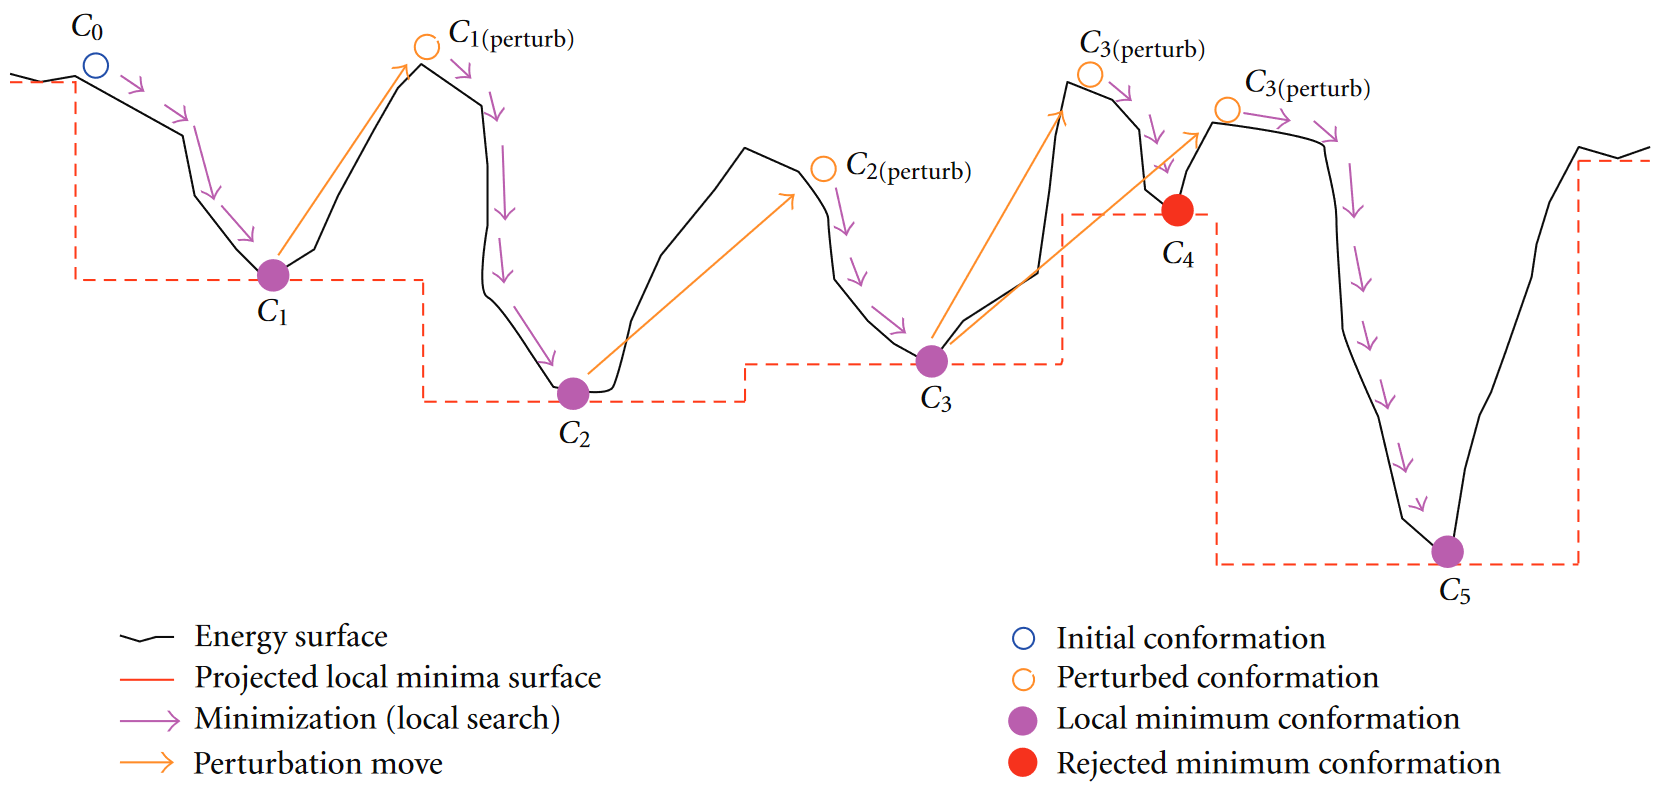
\includegraphics[scale=0.3]{images/7_appendix/bh.png}
    \caption{The Basin-hopping algorithm can be visualized as a transformation of the loss function (black line) into single steps(dotted line). 
    The local optimization routine is illustrated by purple arrows while the random perturbation is represented by yellow arrows. At $C_3$ the perturbation move fails the Metropolis acceptance criterion since the barrier is too high, a new perturbation move to a more favorable position is therefore made. Source: \cite{Olson2012}.}
    \label{fig:Basin-hopping}
\end{figure}

\section{Quartz Sellmeier approximation}
\label{sec:sellmeier}
In \cite{DGrischkowsky1990} the optical parameters along the fast and slow direction of crystalline quartz in the frequency range \SIrange{0.2}{2.0}{\tera\hertz} were published. The result was obtained through a measurement similar to the THz-TDS measurements performed in this work. In order to obtain an interpolation of the refractive indices with a sufficiently high accuracy from the publication we fitted the 3rd order Sellmeier relation which is given by the following expression:

\begin{equation}
    \label{eq:sellmeier}
    n^2(\lambda) - 1 = \frac{A_1\lambda^2}{\lambda^2-B_1}+\frac{A_2\lambda^2}{\lambda^2-B_2}+\frac{A_3\lambda^2}{\lambda^2-B_3},
\end{equation}

where the $A_j$, $B_j$ are fit parameters determined empirically and $\lambda$ is the wavelength in micrometres \cite{Sellmeier1872}. It is worth noting that the same method is used in \cite{Vilas2013} to obtain the wavelength dependency of the refractive indices along the two axes of \ce{MgF2} which are also used for the design development of an AWP. Furthermore, we fitted a polynomial to interpolate the absorption coefficients. The data points obtained from \cite{DGrischkowsky1990} as well as the corresponding fits for the refractive indices and absorption coefficients are shown in figures \ref{fig:ri_quartz} and \ref{fig:abs_quartz} respectively. The fitted Sellemeier coefficients are shown in table \ref{tab:sellmeier_parameters_table}. Since the refractive indices and absorption coefficients of the fast and slow axes are fairly smooth the fits are quite close to the data points. We use these fitted values for the calculations based on the optical parameters of crystalline quartz to reproduce the TAQ design.

\begin{figure}[H]
    \centering
    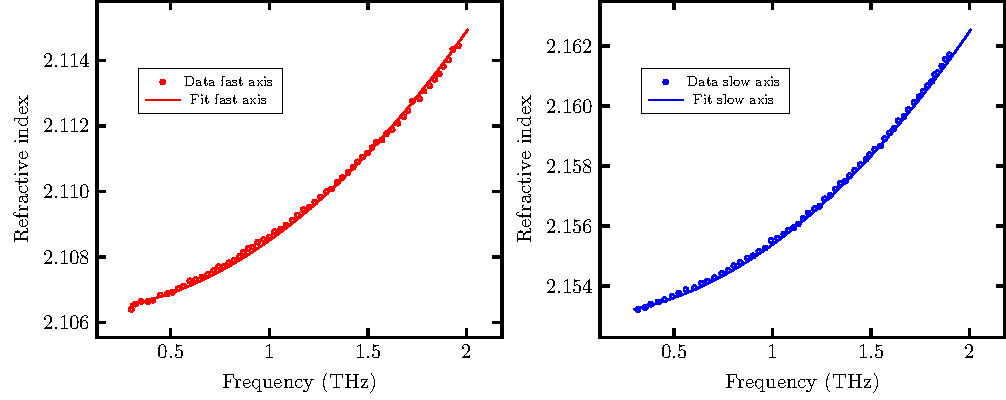
\includegraphics[scale=0.7]{images/7_appendix/plots/quartz_fits/ri_quartz.pdf}
    \caption{Refractive index of crystalline quartz along the fast (left subfigure) and slow (right subfigure) direction. Data points are obtained from \cite{DGrischkowsky1990} and subsequently used to fit the parameters of equation \ref{eq:sellmeier}.}
    \label{fig:ri_quartz}
\end{figure}

\begin{figure}[H]
    \centering
    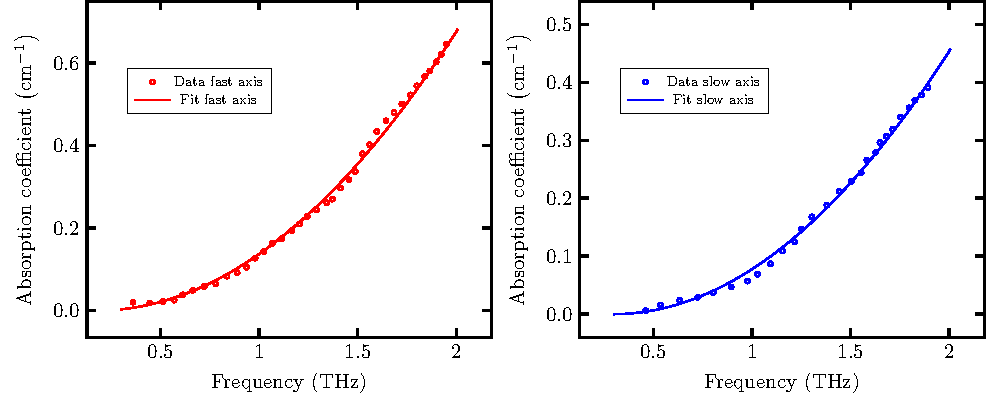
\includegraphics[scale=0.7]{images/7_appendix/plots/quartz_fits/abs_quartz.pdf}
    \caption{Absorption coefficient of crystalline quartz along the fast (left subfigure) and slow (right subfigure) direction. Data points are obtained from \cite{DGrischkowsky1990} which are used to determine the coefficients of a polynomial fit.}
    \label{fig:abs_quartz}
\end{figure}

\begin{table}[H]
    \centering
    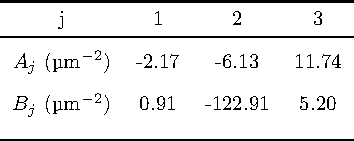
\includegraphics[scale=0.9]{images/7_appendix/sellmeier_parameters_table.pdf}
    \caption{Sellmeier parameters of crystalline quartz obtained from the fit of equation \ref{eq:sellmeier} to the measurement result published in \cite{DGrischkowsky1990}.}
    \label{tab:sellmeier_parameters_table}
\end{table}

\section{Stratified structure CST simulation}
\label{sec:CST simulation}
In order to obtain the form birefringence of a single stratified structure numerically we performed a unit cell simulation in the frequency domain of the structure shown in figure \ref{fig:CST_model}. For this type of simulation the unit cell is assumed to be repeating itself infinitely in the x- and y-direction according to the coordinate system shown in the figure, this saves a lot of memory and computing time and is nevertheless a good model of the real structure. The lower part of the unit cell (light blue) represents the material which in this case is modeled using the measured optical parameters of HIPS and the upper part represents the air gap ($n=1$, dark blue). To model the grating the height (y-direction) of the HIPS and air layer is therefore $a=\SI{735}{\micro \meter}$ and $b=\SI{393}{\micro \meter}$ respectively. The thickness of the grating $d$ is measured by the z-coordinate and is variable. 

\begin{figure}[H]
    \centering
    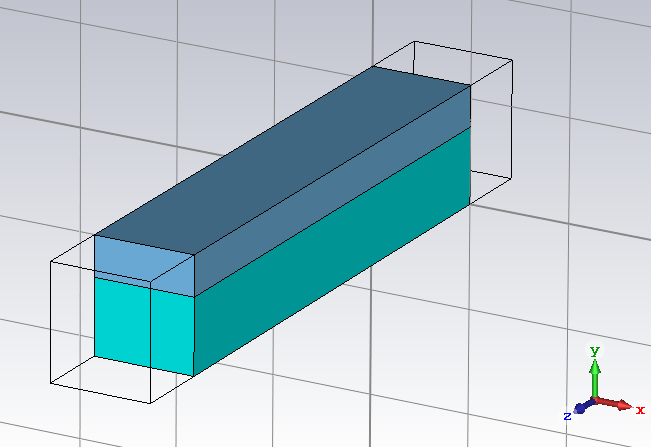
\includegraphics[scale=0.3]{images/7_appendix/CST.PNG}
    \caption{Unit cell of the structure representing a stratified medium with $a=\SI{735}{\micro \meter}$ and $b=\SI{393}{\micro \meter}$.}
    \label{fig:CST_model}
\end{figure}

This means that if we assume that the structure is birefringent and the incoming radiation is linearly polarized at \SI{45}{\degree} then for some frequency we expect that the magnitude of the field perpendicular to the input given by $|S_{21}|$ attains a minimum. In other words the effect of a half waveplate which means that equation \ref{eq:thickness_half_waveplate} is satisfied and we can rewrite it as follows:
\begin{equation}
    \frac{2d}{\lambda_0}=|n_o-n_e|=\Delta n,
\end{equation}
where we assume that the order is zero. Therefore, varying $d$ in small steps and determining $\lambda_0=\argmin|S_{21}(\lambda)|$ we can obtain the birefringence at $\lambda_0$. Figure \ref{fig:bf_sim} shows $|S_{21}|$ as a function of the frequency for the integer values of $d$.

\begin{figure}[H]
    \centering
    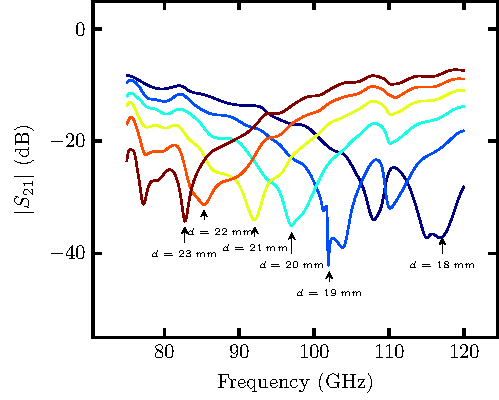
\includegraphics[scale=1]{images/7_appendix/plots/cst_sim/bf_sim.pdf}
    \caption{$|S_{21}|$ as a function of frequency obtained through the simulation of the unit cell shown in figure \ref{fig:CST_model} for different thicknesses of the structure.}
    \label{fig:bf_sim}
\end{figure}

\chapter{Characterization of ceramic material samples}
%\setcounter{page}{1} % remove in thesis version
\label{sec:ceramic_characterization}
\section{Description}
The 10 different material samples shown in figure \ref{fig:ceramic_samples} were characterized regarding their birefringence. To that extend each sample was placed in the focus of the two leftmost off axis parabolic mirrors as shown in figure \ref{fig:THz-TDS-HHI} (a). The sample holder is shown in figure \ref{fig:THz-TDS-HHI} (b) which enables a \SI{360}{\degree} manual rotation of the sample in the direction of the red arrow. The blue arrow in (a) and (b) indicates the polarization plane of the incident THz pulse. Each sample was placed in the holder so that the printing direction was approximately aligned with the \SI{0}{\degree} and \SI{180}{\degree} direction. Some samples were without a flat side but instead had an arrow drawn on them. In those cases we aligned the arrow so that it was parallel to the polarization of the THz radiation. At \SI{0}{\degree} the polarization plane and the printing direction of the 10 samples therefore align and at \SI{90}{\degree} they are orthogonal as shown in (b). 

\begin{figure}
    \centering
    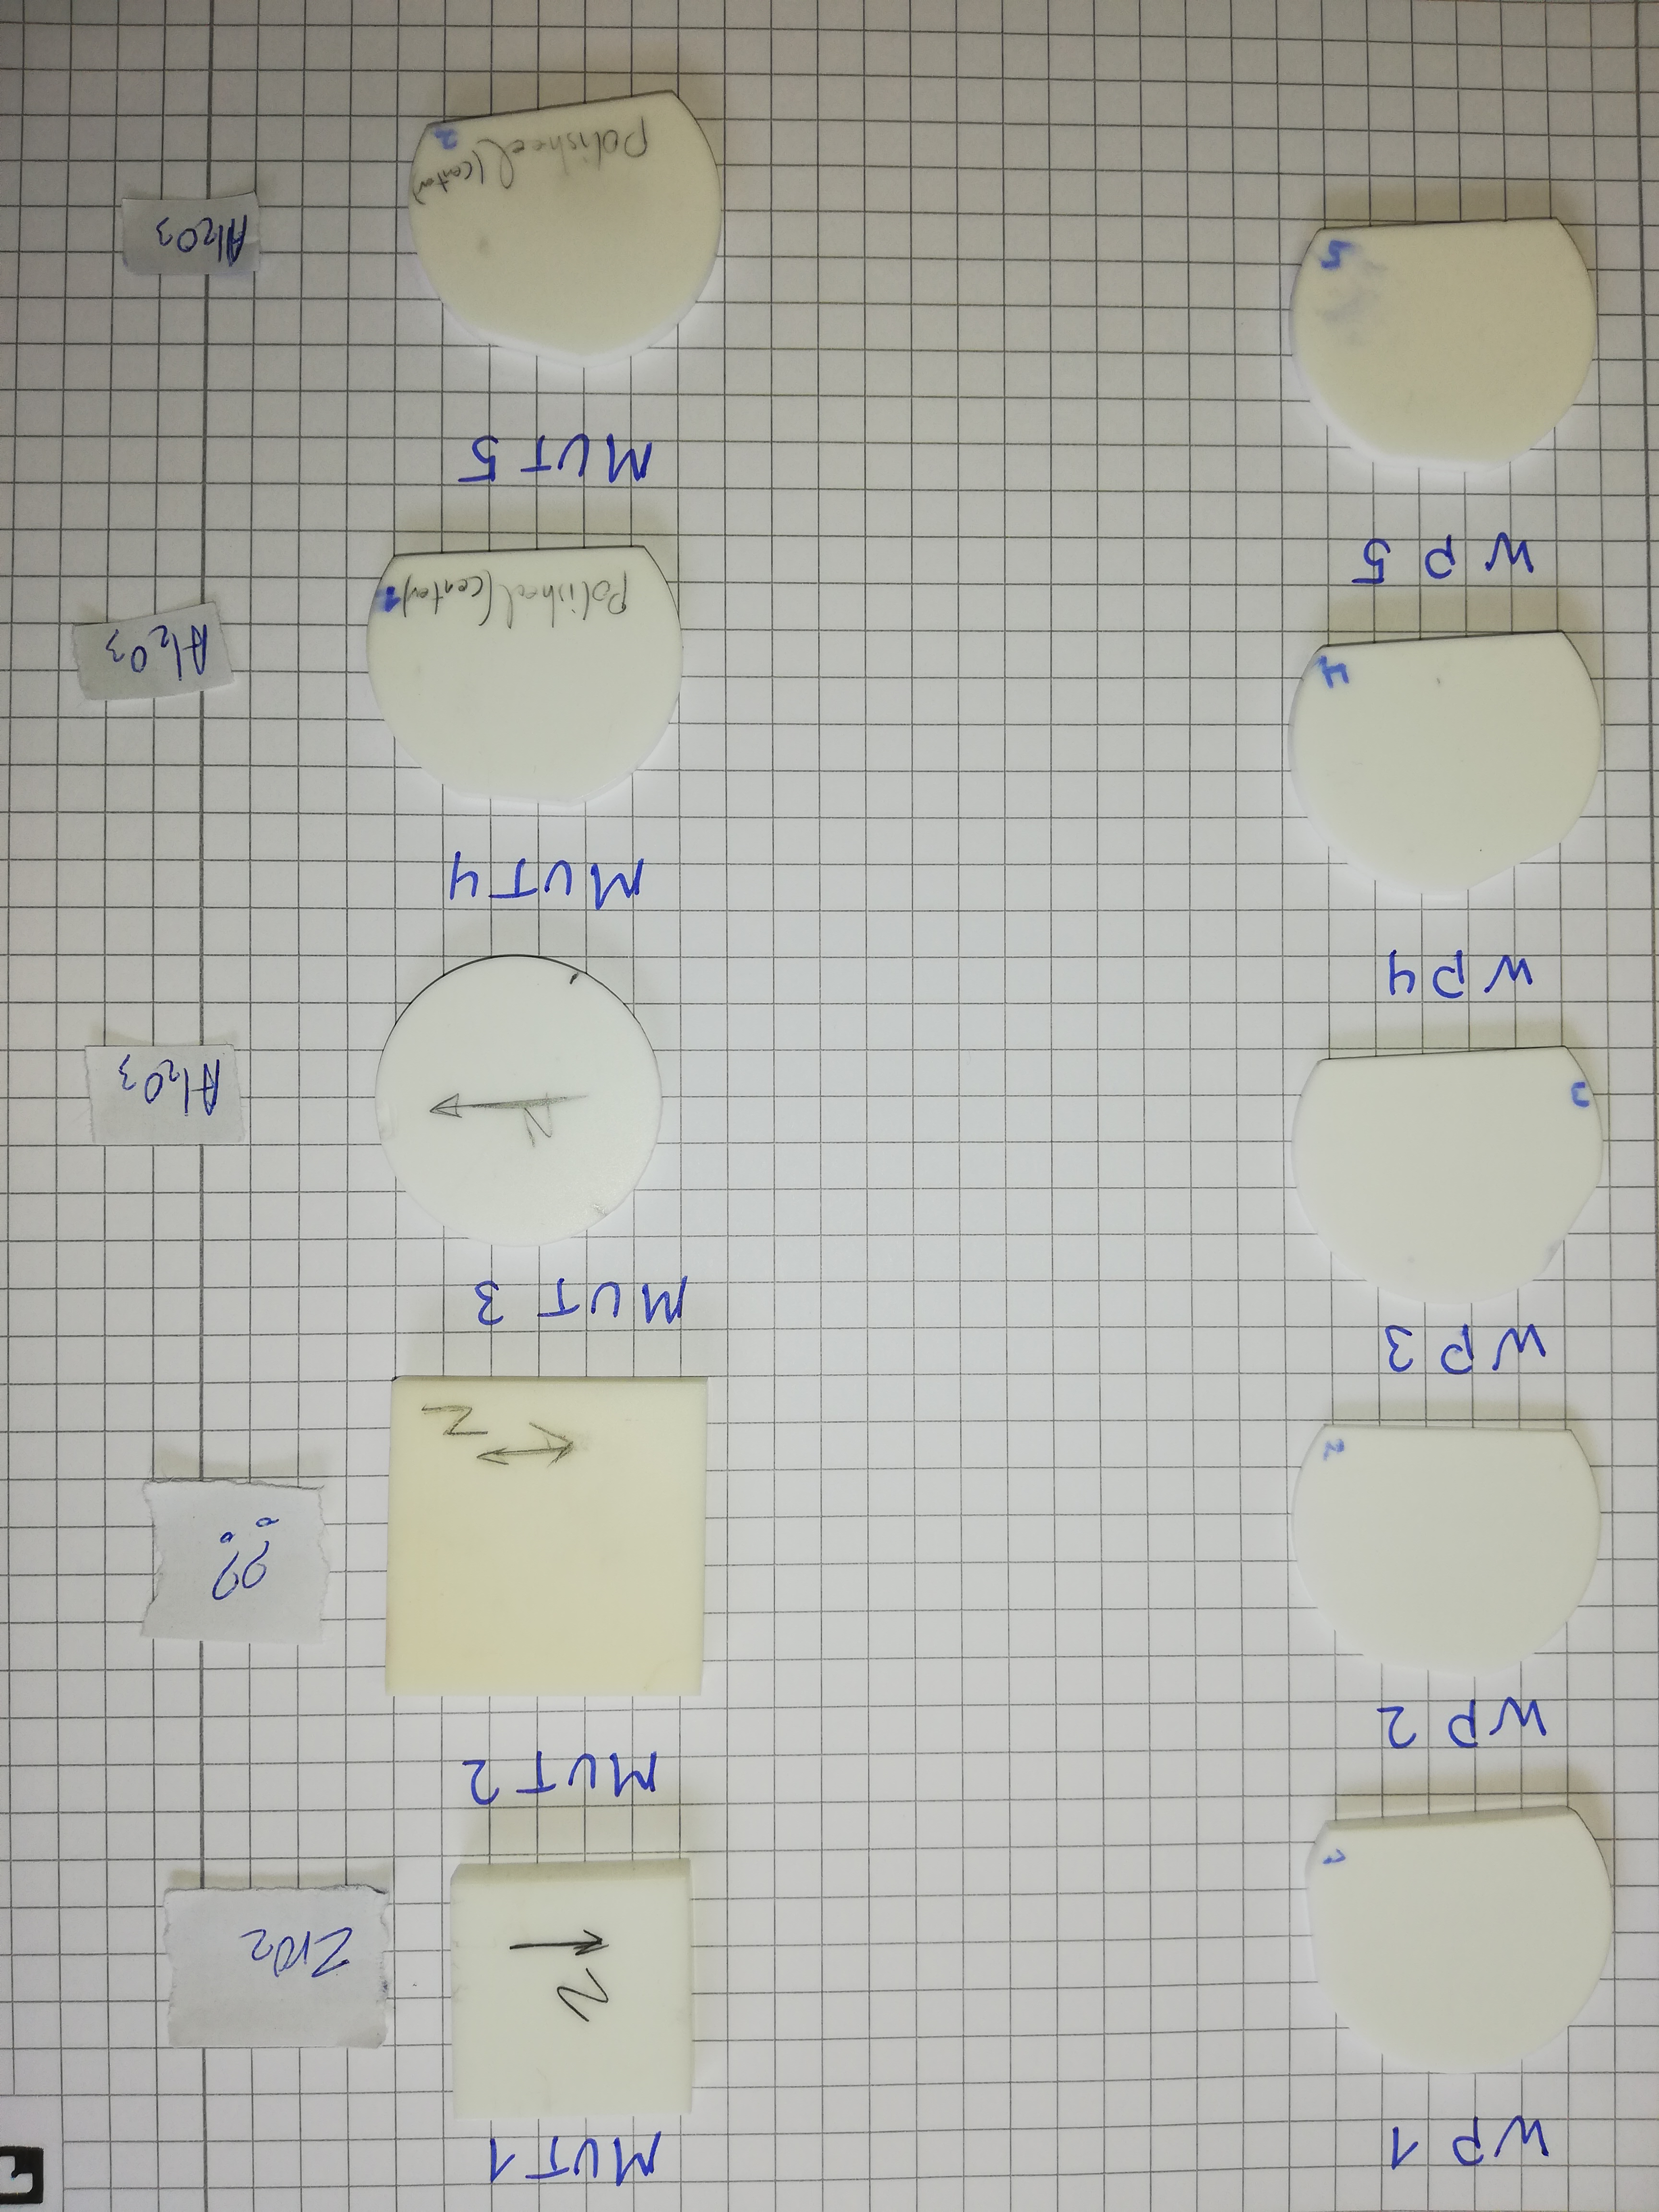
\includegraphics[scale=0.1,angle=180,origin=c]{images/7_appendix/ceramic_samples.jpg}
    \caption{Photo of the 10 characterized samples}
    \label{fig:ceramic_samples}
\end{figure}

\begin{figure}[H]
    \centering
    \subcaptionbox{\label{fig:setup_1}}
        {\hspace*{-2em}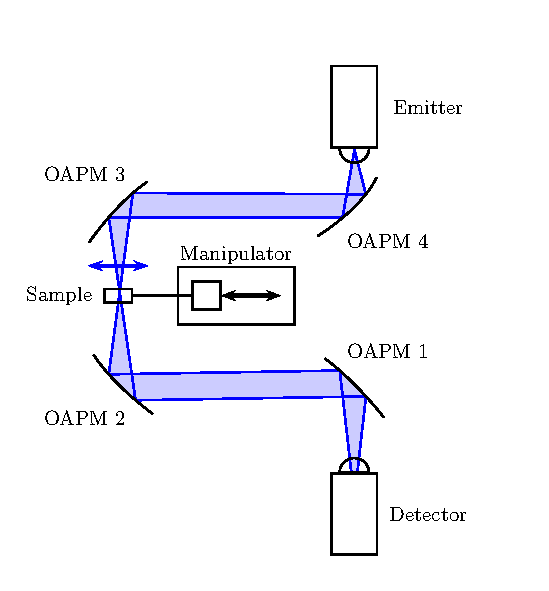
\includegraphics[width=0.45\linewidth]{images/7_appendix/Setup-THz-TDS-HHI.pdf}}
    \qquad
    \subcaptionbox{\label{fig:setup_2}}
        {\hspace*{-2em}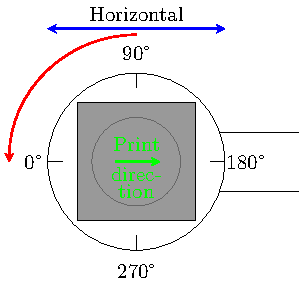
\includegraphics[width=0.45\linewidth]{images/7_appendix/sample_mount.pdf}}
    
    \caption{Subfigure (a): Main components of the measurement setup which consists of four off axis parabolic mirros, the sample mounted on a translation stage(manipulator) as well as the emitter and detector. Subfigure (b): Sample placed on a rotational mount. The blue arrow indicates the horizontal direction which is also the polarization plane of the incident radiation. The red arrow indicates the turn direction and the green arrow the direction in which the sample was printed.}
    \label{fig:THz-TDS-HHI}
\end{figure}

Each measurement was taken with a relative humidity of less than \SI{1}{\percent} and a mechanical stage was used to move the sample out of the beam path for a reference measurement. Due to the relative long nitrogen purge time and the manual sample rotator we measured each sample at three angles; \SI{0}{\degree}, \SI{90}{\degree} and \SI{180}{\degree}.
Table \ref{tab:ceramic_samples_table} lists the 10 samples, their respective handles which is used later and their respective measured thickness. The thickness was determined approximately at the center of each sample using a micrometer screw gauge. This thickness was then used for extraction of the refractive index for all three sample orientations. 

\begin{table}[h]
    \centering
    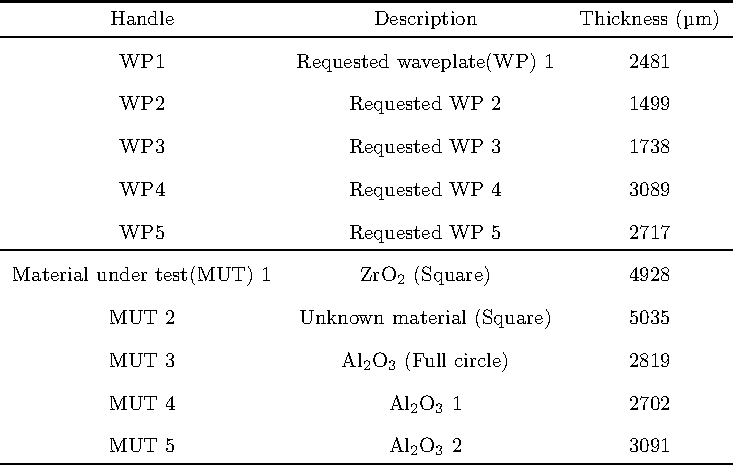
\includegraphics[scale=1.0]{images/7_appendix/ceramic_samples_table.pdf}
    \caption{The 10 characterized samples. The first five are the samples requested for the achromatic waveplate while the five in the lower half are the additionally characterized samples. The thickness is measured once at the center of the each sample using a micrometer.}
    \label{tab:ceramic_samples_table}
\end{table}

\newpage

\section{Results}
The data collected from the measurements was evaluated using the commercial software Teralyzer. We used the same thickness for all three angles for a given sample to be able to compare the refractive index at the three different rotational angles. The thicknesses used for the evaluation of each sample is given in \ref{tab:ceramic_samples_table}. 
It is possible to leave the thickness as a free parameter which can then be fitted and thereby slightly adjusted for each measurement to remove or reduce the oscillations seen in for example WP2 at \SI{0}{\degree}. Although, this introduces a slight frequency independent offset in the refractive index which depends on the fitted thickness and thereby changes the measured birefringence. We therefore chose to use one thickness for all three angles. 

Figure \ref{fig:ceramic_WPs} shows the evaluated refractive index at the three angles for the requested waveplates 1-5 and figure \ref{fig:ceramic_MUTs} shows the results of the evaluation for the additional five samples. The strong attenuation of MUT1 limited the usable frequency range to \SI{0.8}{\tera \hertz}. 

\begin{figure}[H]
\centering
\subcaptionbox{\label{fig:ceramic_WP1}}
    {\hspace*{-2em}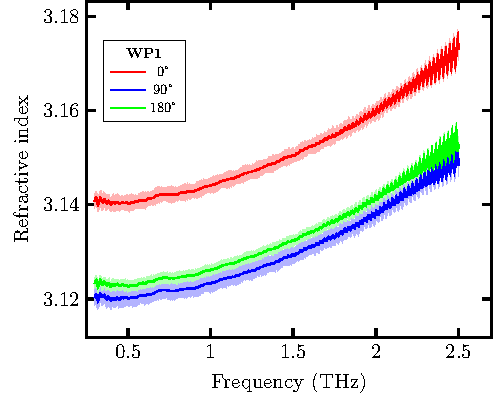
\includegraphics[width=0.45\linewidth]{images/7_appendix/plots/real/WP1.pdf}}
\qquad
\subcaptionbox{\label{fig:ceramic_WP2}}
    {\hspace*{-2em}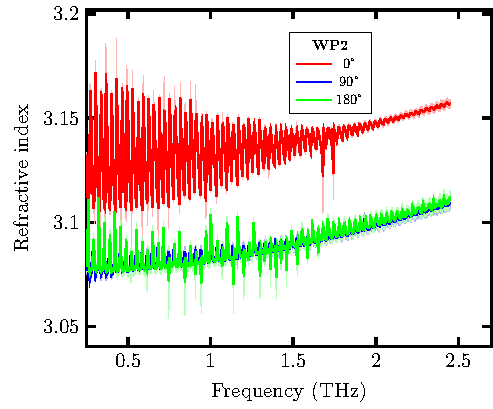
\includegraphics[width=0.45\linewidth]{images/7_appendix/plots/real/WP2.pdf}}
\subcaptionbox{\label{fig:ceramic_WP3}}
    {\hspace*{-2em}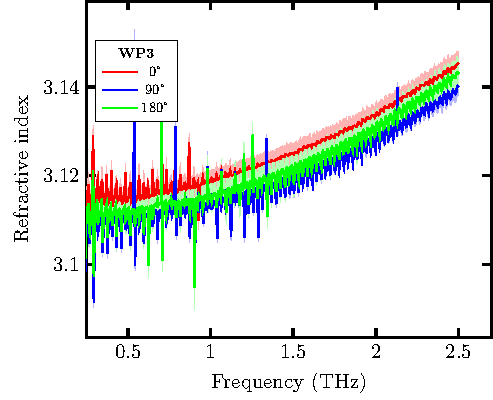
\includegraphics[width=0.45\linewidth]{images/7_appendix/plots/real/WP3.pdf}}
\qquad
\subcaptionbox{\label{fig:ceramic_WP4}}
    {\hspace*{-2em}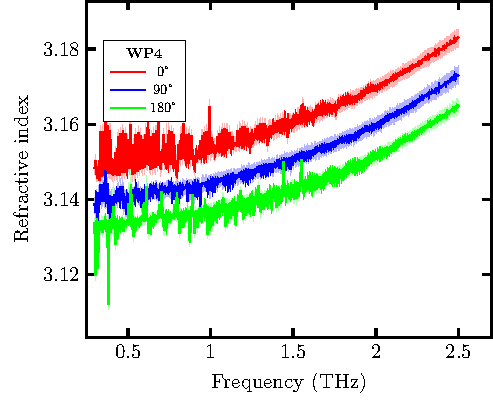
\includegraphics[width=0.45\linewidth]{images/7_appendix/plots/real/WP4.pdf}}
\subcaptionbox{\label{fig:ceramic_WP5}}
    {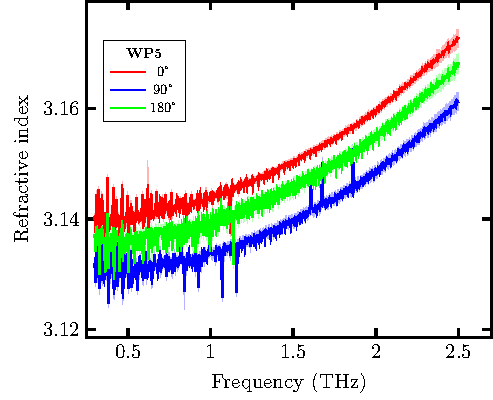
\includegraphics[width=0.45\linewidth]{images/7_appendix/plots/real/WP5.pdf}}
\caption{Evaluated refractive index for the five requested waveplates at three different rotational angles.}
\label{fig:ceramic_WPs}
\end{figure}

\begin{figure}[H]
\centering
\subcaptionbox{\label{fig:ceramic_MUT1}}
    {\hspace*{-2em}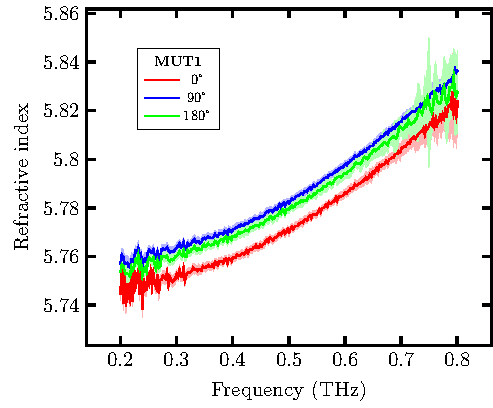
\includegraphics[width=0.45\linewidth]{images/7_appendix/plots/real/MUT1.pdf}}
\qquad
\subcaptionbox{\label{fig:ceramic_MUT2}}
    {\hspace*{-2em}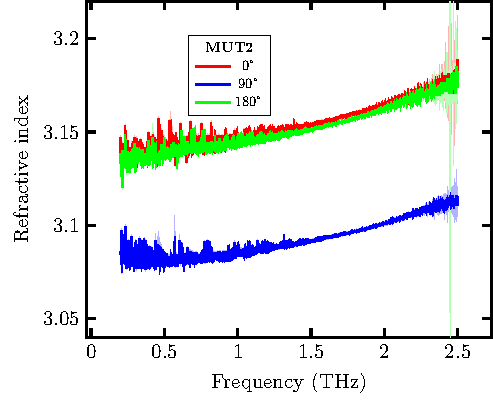
\includegraphics[width=0.45\linewidth]{images/7_appendix/plots/real/MUT2.pdf}}
\subcaptionbox{\label{fig:ceramic_MUT3}}
    {\hspace*{-2em}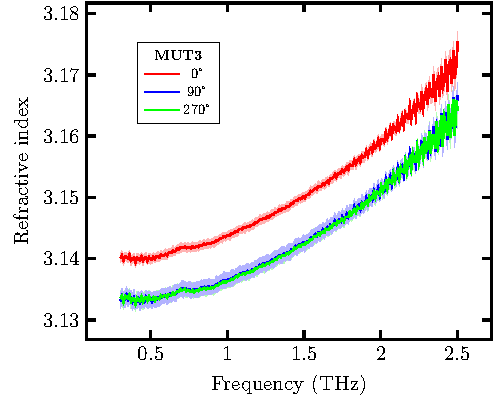
\includegraphics[width=0.45\linewidth]{images/7_appendix/plots/real/MUT3.pdf}}
\qquad
\subcaptionbox{\label{fig:ceramic_MUT4}}
    {\hspace*{-2em}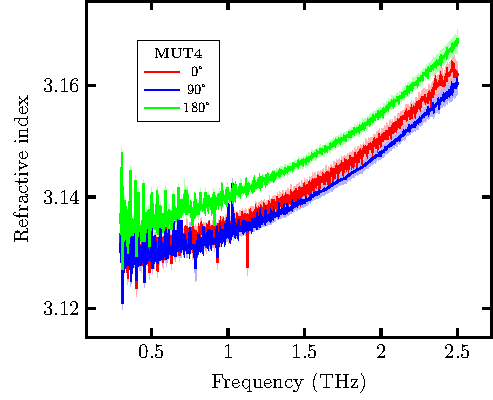
\includegraphics[width=0.45\linewidth]{images/7_appendix/plots/real/MUT4.pdf}}
\subcaptionbox{\label{fig:ceramic_MUT5}}
    {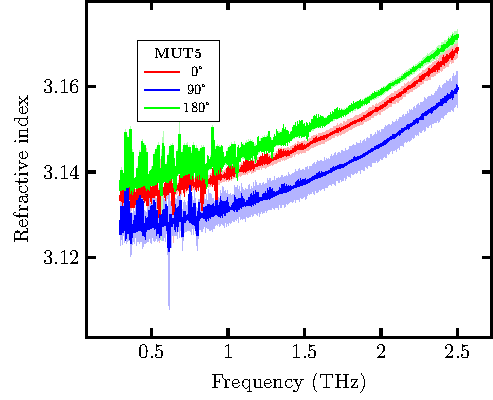
\includegraphics[width=0.45\linewidth]{images/7_appendix/plots/real/MUT5.pdf}}
\caption{Evaluated refractive index for the five additional samples at three different rotational angles.}
\label{fig:ceramic_MUTs}
\end{figure}

\begin{figure}[H]
\centering
\subcaptionbox{\label{fig:ceramic_WP1_abs}}
    {\hspace*{-2em}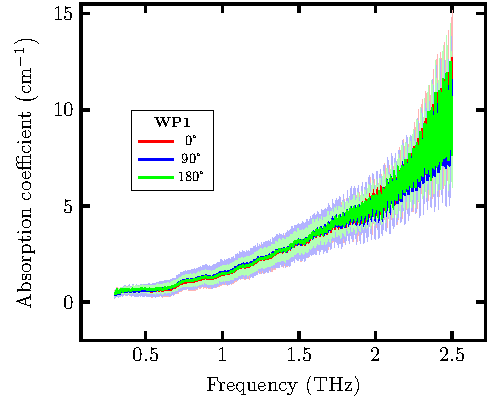
\includegraphics[width=0.45\linewidth]{images/7_appendix/plots/real_abs/WP1.pdf}}
\qquad
\subcaptionbox{\label{fig:ceramic_WP2_abs}}
    {\hspace*{-2em}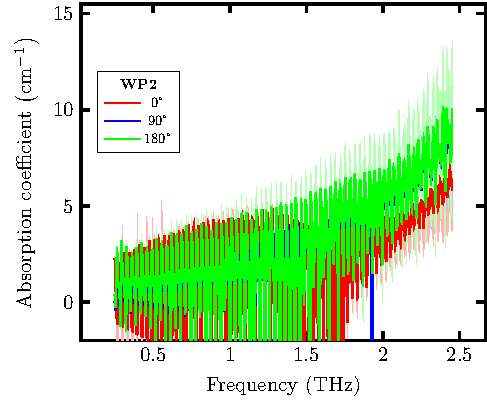
\includegraphics[width=0.45\linewidth]{images/7_appendix/plots/real_abs/WP2.pdf}}
\subcaptionbox{\label{fig:ceramic_WP3_abs}}
    {\hspace*{-2em}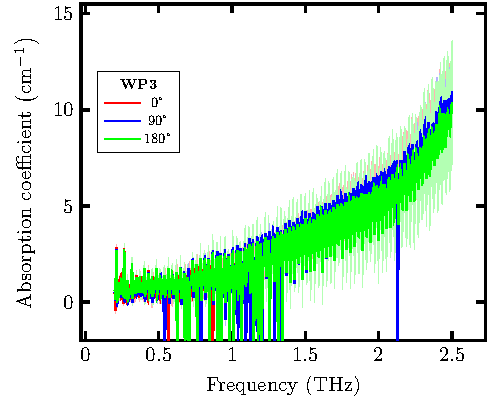
\includegraphics[width=0.45\linewidth]{images/7_appendix/plots/real_abs/WP3.pdf}}
\qquad
\subcaptionbox{\label{fig:ceramic_WP4_abs}}
    {\hspace*{-2em}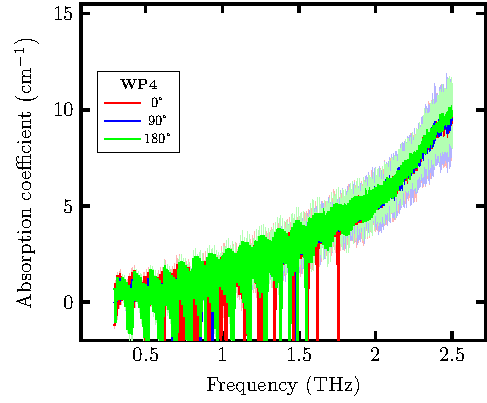
\includegraphics[width=0.45\linewidth]{images/7_appendix/plots/real_abs/WP4.pdf}}
\subcaptionbox{\label{fig:ceramic_WP5_abs}}
    {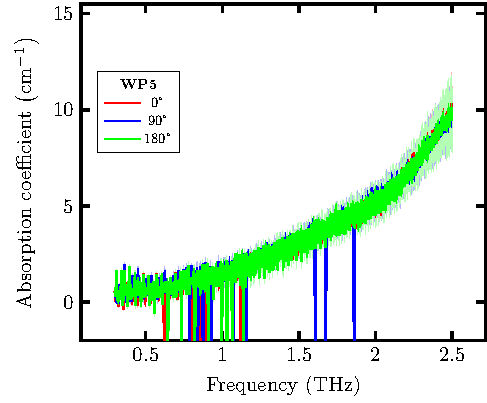
\includegraphics[width=0.45\linewidth]{images/7_appendix/plots/real_abs/WP5.pdf}}
\caption{Evaluated absorption coefficient for the five requested waveplates at three different rotational angles.}
\label{fig:ceramic_WPs_abs}
\end{figure}

\begin{figure}[H]
\centering
\subcaptionbox{\label{fig:ceramic_MUT1_abs}}
    {\hspace*{-2em}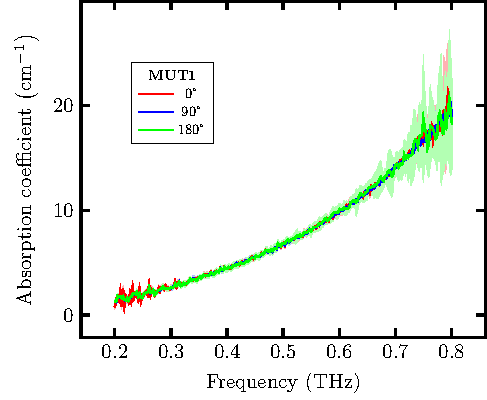
\includegraphics[width=0.45\linewidth]{images/7_appendix/plots/real_abs/MUT1.pdf}}
\qquad
\subcaptionbox{\label{fig:ceramic_MUT2_abs}}
    {\hspace*{-2em}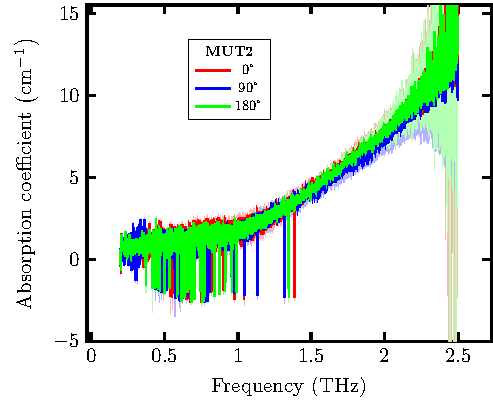
\includegraphics[width=0.45\linewidth]{images/7_appendix/plots/real_abs/MUT2.pdf}}
\subcaptionbox{\label{fig:ceramic_MUT3_abs}}
    {\hspace*{-2em}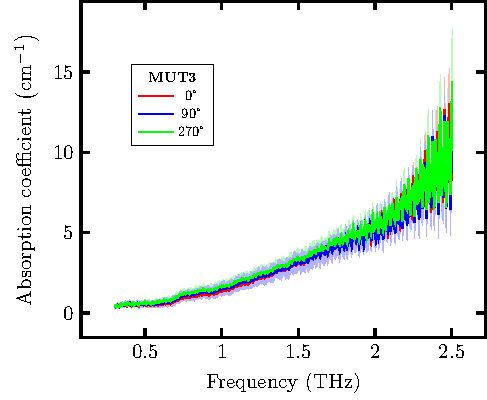
\includegraphics[width=0.45\linewidth]{images/7_appendix/plots/real_abs/MUT3.pdf}}
\qquad
\subcaptionbox{\label{fig:ceramic_MUT4_abs}}
    {\hspace*{-2em}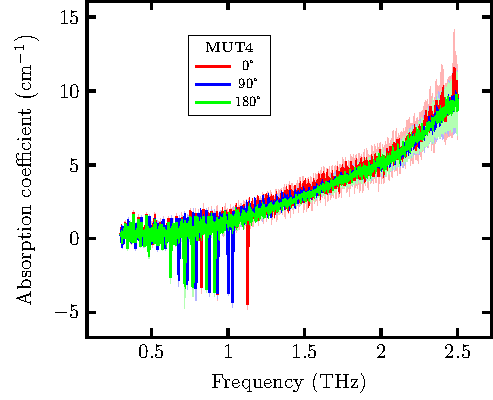
\includegraphics[width=0.45\linewidth]{images/7_appendix/plots/real_abs/MUT4.pdf}}
\subcaptionbox{\label{fig:ceramic_MUT5_abs}}
    {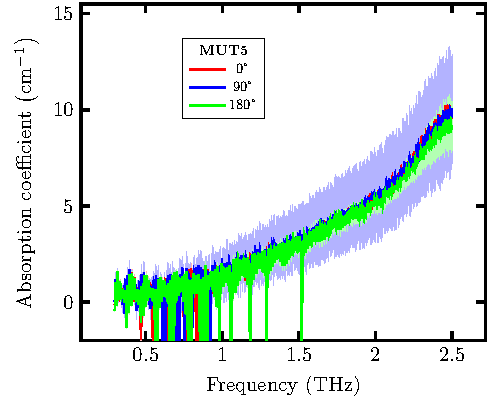
\includegraphics[width=0.45\linewidth]{images/7_appendix/plots/real_abs/MUT5.pdf}}
\caption{Evaluated absorption coefficient for the five additional samples at three different rotational angles.}
\label{fig:ceramic_MUTs_abs}
\end{figure}

If we compare the measured refractive index and the absorption coefficient of these \ce{Al2O3} samples to the result from the measurement published in \cite{Ornik2018} of two similar \ce{Al2O3} samples, we see that the refractive index and absorption coefficient for WP1-WP5 and MUT3-MUT5 is approximately the same. Furthermore, we see that the refractive index and absorption coefficient of MUT1 is higher than the other samples since this sample consists of \ce{ZrO2}. The material of MUT2 was either \ce{ZrO2} or \ce{Al2O3}, based on the value of the refractive index we can conclude that MUT2 consists of \ce{Al2O3}. Finally, it seems that none of the samples have a measurable birefringence except MUT2 which has a birefringence of around $0.05$. The missing birefringence could be due to a different printing process and or different printing settings.


\printbibliography

% phew
\end{document}
